\documentclass[a4paper,11pt]{article}
\usepackage[a4paper, margin=8em]{geometry}

% usa i pacchetti per la scrittura in italiano
\usepackage[french,italian]{babel}
\usepackage[T1]{fontenc}
\usepackage[utf8]{inputenc}
\frenchspacing 

% usa i pacchetti per la formattazione matematica
\usepackage{amsmath, amssymb, amsthm, amsfonts}

% usa altri pacchetti
\usepackage{gensymb}
\usepackage{hyperref}
\usepackage{standalone}

\usepackage{colortbl}

\usepackage{xstring}
\usepackage{karnaugh-map}

% imposta il titolo
\title{Appunti Ingegneria del Software}
\author{Luca Seggiani}
\date{2025}

% imposta lo stile
% usa helvetica
\usepackage[scaled]{helvet}
% usa palatino
\usepackage{palatino}
% usa un font monospazio guardabile
\usepackage{lmodern}

\renewcommand{\rmdefault}{ppl}
\renewcommand{\sfdefault}{phv}
\renewcommand{\ttdefault}{lmtt}

% circuiti
\usepackage{circuitikz}
\usetikzlibrary{babel}

% testo cerchiato
\newcommand*\circled[1]{\tikz[baseline=(char.base)]{
            \node[shape=circle,draw,inner sep=2pt] (char) {#1};}}

% disponi il titolo
\makeatletter
\renewcommand{\maketitle} {
	\begin{center} 
		\begin{minipage}[t]{.8\textwidth}
			\textsf{\huge\bfseries \@title} 
		\end{minipage}%
		\begin{minipage}[t]{.2\textwidth}
			\raggedleft \vspace{-1.65em}
			\textsf{\small \@author} \vfill
			\textsf{\small \@date}
		\end{minipage}
		\par
	\end{center}

	\thispagestyle{empty}
	\pagestyle{fancy}
}
\makeatother

% disponi teoremi
\usepackage{tcolorbox}
\newtcolorbox[auto counter, number within=section]{theorem}[2][]{%
	colback=blue!10, 
	colframe=blue!40!black, 
	sharp corners=northwest,
	fonttitle=\sffamily\bfseries, 
	title=Teorema~\thetcbcounter: #2, 
	#1
}

% disponi definizioni
\newtcolorbox[auto counter, number within=section]{definition}[2][]{%
	colback=red!10,
	colframe=red!40!black,
	sharp corners=northwest,
	fonttitle=\sffamily\bfseries,
	title=Definizione~\thetcbcounter: #2,
	#1
}

% disponi codice
\usepackage{listings}
\usepackage[table]{xcolor}

\definecolor{codegreen}{rgb}{0,0.6,0}
\definecolor{codegray}{rgb}{0.5,0.5,0.5}
\definecolor{codepurple}{rgb}{0.58,0,0.82}
\definecolor{backcolour}{rgb}{0.95,0.95,0.92}

\lstdefinestyle{codestyle}{
		backgroundcolor=\color{black!5}, 
		commentstyle=\color{codegreen},
		keywordstyle=\bfseries\color{magenta},
		numberstyle=\sffamily\tiny\color{black!60},
		stringstyle=\color{green!50!black},
		basicstyle=\ttfamily\footnotesize,
		breakatwhitespace=false,         
		breaklines=true,                 
		captionpos=b,                    
		keepspaces=true,                 
		numbers=left,                    
		numbersep=5pt,                  
		showspaces=false,                
		showstringspaces=false,
		showtabs=false,                  
		tabsize=2
}

\lstdefinestyle{shellstyle}{
		backgroundcolor=\color{black!5}, 
		basicstyle=\ttfamily\footnotesize\color{black}, 
		commentstyle=\color{black}, 
		keywordstyle=\color{black},
		numberstyle=\color{black!5},
		stringstyle=\color{black}, 
		showspaces=false,
		showstringspaces=false, 
		showtabs=false, 
		tabsize=2, 
		numbers=none, 
		breaklines=true
}


\lstdefinelanguage{assembler}{ 
  keywords={AAA, AAD, AAM, AAS, ADC, ADCB, ADCW, ADCL, ADD, ADDB, ADDW, ADDL, AND, ANDB, ANDW, ANDL,
        ARPL, BOUND, BSF, BSFL, BSFW, BSR, BSRL, BSRW, BSWAP, BT, BTC, BTCB, BTCW, BTCL, BTR, 
        BTRB, BTRW, BTRL, BTS, BTSB, BTSW, BTSL, CALL, CBW, CDQ, CLC, CLD, CLI, CLTS, CMC, CMP,
        CMPB, CMPW, CMPL, CMPS, CMPSB, CMPSD, CMPSW, CMPXCHG, CMPXCHGB, CMPXCHGW, CMPXCHGL,
        CMPXCHG8B, CPUID, CWDE, DAA, DAS, DEC, DECB, DECW, DECL, DIV, DIVB, DIVW, DIVL, ENTER,
        HLT, IDIV, IDIVB, IDIVW, IDIVL, IMUL, IMULB, IMULW, IMULL, IN, INB, INW, INL, INC, INCB,
        INCW, INCL, INS, INSB, INSD, INSW, INT, INT3, INTO, INVD, INVLPG, IRET, IRETD, JA, JAE,
        JB, JBE, JC, JCXZ, JE, JECXZ, JG, JGE, JL, JLE, JMP, JNA, JNAE, JNB, JNBE, JNC, JNE, JNG,
        JNGE, JNL, JNLE, JNO, JNP, JNS, JNZ, JO, JP, JPE, JPO, JS, JZ, LAHF, LAR, LCALL, LDS,
        LEA, LEAVE, LES, LFS, LGDT, LGS, LIDT, LMSW, LOCK, LODSB, LODSD, LODSW, LOOP, LOOPE,
        LOOPNE, LSL, LSS, LTR, MOV, MOVB, MOVW, MOVL, MOVSB, MOVSD, MOVSW, MOVSX, MOVSXB,
        MOVSXW, MOVSXL, MOVZX, MOVZXB, MOVZXW, MOVZXL, MUL, MULB, MULW, MULL, NEG, NEGB, NEGW,
        NEGL, NOP, NOT, NOTB, NOTW, NOTL, OR, ORB, ORW, ORL, OUT, OUTB, OUTW, OUTL, OUTSB, OUTSD,
        OUTSW, POP, POPL, POPW, POPB, POPA, POPAD, POPF, POPFD, PUSH, PUSHL, PUSHW, PUSHB, PUSHA, 
				PUSHAD, PUSHF, PUSHFD, RCL, RCLB, RCLW, MOVSL, MOVSB, MOVSW, STOSL, STOSB, STOSW, LODSB, LODSW,
				LODSL, INSB, INSW, INSL, OUTSB, OUTSL, OUTSW
        RCLL, RCR, RCRB, RCRW, RCRL, RDMSR, RDPMC, RDTSC, REP, REPE, REPNE, RET, ROL, ROLB, ROLW,
        ROLL, ROR, RORB, RORW, RORL, SAHF, SAL, SALB, SALW, SALL, SAR, SARB, SARW, SARL, SBB,
        SBBB, SBBW, SBBL, SCASB, SCASD, SCASW, SETA, SETAE, SETB, SETBE, SETC, SETE, SETG, SETGE,
        SETL, SETLE, SETNA, SETNAE, SETNB, SETNBE, SETNC, SETNE, SETNG, SETNGE, SETNL, SETNLE,
        SETNO, SETNP, SETNS, SETNZ, SETO, SETP, SETPE, SETPO, SETS, SETZ, SGDT, SHL, SHLB, SHLW,
        SHLL, SHLD, SHR, SHRB, SHRW, SHRL, SHRD, SIDT, SLDT, SMSW, STC, STD, STI, STOSB, STOSD,
        STOSW, STR, SUB, SUBB, SUBW, SUBL, TEST, TESTB, TESTW, TESTL, VERR, VERW, WAIT, WBINVD,
        XADD, XADDB, XADDW, XADDL, XCHG, XCHGB, XCHGW, XCHGL, XLAT, XLATB, XOR, XORB, XORW, XORL},
  keywordstyle=\color{blue}\bfseries,
  ndkeywordstyle=\color{darkgray}\bfseries,
  identifierstyle=\color{black},
  sensitive=false,
  comment=[l]{\#},
  morecomment=[s]{/*}{*/},
  commentstyle=\color{purple}\ttfamily,
  stringstyle=\color{red}\ttfamily,
  morestring=[b]',
  morestring=[b]"
}

\lstset{language=assembler, style=codestyle}

% disponi sezioni
\usepackage{titlesec}

\titleformat{\section}
	{\sffamily\Large\bfseries} 
	{\thesection}{1em}{} 
\titleformat{\subsection}
	{\sffamily\large\bfseries}   
	{\thesubsection}{1em}{} 
\titleformat{\subsubsection}
	{\sffamily\normalsize\bfseries} 
	{\thesubsubsection}{1em}{}

% tikz
\usepackage{tikz}

% float
\usepackage{float}

% grafici
\usepackage{pgfplots}
\pgfplotsset{width=10cm,compat=1.9}

% disponi alberi
\usepackage{forest}

\forestset{
	rectstyle/.style={
		for tree={rectangle,draw,font=\large\sffamily}
	},
	roundstyle/.style={
		for tree={circle,draw,font=\large}
	}
}

% disponi algoritmi
\usepackage{algorithm}
\usepackage{algorithmic}
\makeatletter
\renewcommand{\ALG@name}{Algoritmo}
\makeatother

% disponi numeri di pagina
\usepackage{fancyhdr}
\fancyhf{} 
\fancyfoot[L]{\sffamily{\thepage}}

\makeatletter
\fancyhead[L]{\raisebox{1ex}[0pt][0pt]{\sffamily{\@title \ \@date}}} 
\fancyhead[R]{\raisebox{1ex}[0pt][0pt]{\sffamily{\@author}}}
\makeatother

\begin{document}
% sezione (data)
\section{Lezione del 26-09-25}

% stili pagina
\thispagestyle{empty}
\pagestyle{fancy}

% testo
\subsection{Introduzione all'UML}
L'\textbf{UML} (\textit{Unified Modeling Language}) è una notazione grafica standardizzata, aperta ed estensibile, di modellazione. 
L'UML è pensato per modellizzare progetti che sfruttano la programmazione ad oggetti (OOP).

Viene detto \textit{unificato} in quanto accompagna il software in tutti i suoi cicli di vita, dalle specifiche all'implementazione.
Può essere usato per modellare diversi domini applicativi (dall'embedded alle applicazioni, ecc...), ed è trasparente al linguaggio e alle metodologie usate.

I modelli di UML rappresentano collezioni di \textbf{oggetti} \textit{interagenti}. In particolare sfruttiamo modelli:
\begin{itemize}
	\item A \textbf{struttura statica}, cioè che dettagliano quali oggetti compongono il nostro progetto in maniera statica;
	\item A \textbf{comportamento dinamico}, cioè dettagliamo successivamente come questi oggetti interagiscono fra loro nel tempo.
\end{itemize}

\subsection{Introduzione all'UP}
L'\textbf{UP} (\textit{Unified Process}) è un processo di ingegnerizzazione software basato su 3 principi fondamentali:
\begin{enumerate}
	\item Guidato dall'analisi dei \textit{requisiti} e dei \textit{rischi};
	\item Centrato sull'\textit{architettura}, cioè finalizzato alla produzione di un'architettura robusta;
	\item \textit{Iterativo} ed \textit{incrementale}, cioè suddivide il progetto in iterazioni incrementali che arrivano da zero al sistema funzionante.
\end{enumerate}

Ciascuna iterazione è finalizzata a uno o più \textit{sotto-obiettivi}: 
\begin{itemize}
	\item Pianificazione;
	\item Analisi e progetto;
	\item Costruzione;
	\item Integrazione e test;
	\item Release interna o esterna.
\end{itemize}

Ogni iterazione genera la cosiddetta \textit{baseline}, cioè la versione da cui partira la prossima iterazione, e via dicendo.
L'\textit{incremento} sarà rappresentato dalla variazione da una baseline alla successiva.

Le fasi vengono implementate seguendo sostanzialmente uno o più fra 5 workflow riassunti dalla sigla \textbf{RADIT}:
\begin{itemize}
	\item \textbf{Requirements} (requisiti);
	\item \textbf{Analysis} (analisi);
	\item \textbf{Design} (design);
	\item \textbf{Implementation} (implementazione);
	\item \textbf{Test} (test).
\end{itemize}

\subsubsection{Struttura dell'UP}
Il ciclo di vita del progetto si evolve in più iterazioni (ciascuna delle quali comprende i 5 workflow RADIT)
.
In particolare individuiamo 4 fasi:
\begin{enumerate}
	\item \textbf{Inception} (principio): qui l'obiettivo è far partire il progetto. Dobbiamo quindi stabilire la \textit{fattibilità} del progetto, creare un caso di business (cioè dimostrare la reddittività del progetto), catturare le specifiche di base ed individuare i primi rischi critici. 

		Gli workflow principali saranno requisiti ed analisi. 

		Vediamo quelle che sono le \textit{milestone} associate a questa fase: vogliamo stabilire un'associazione fra \textit{condizioni} da soddisfare e \textbf{deliverable} (\textit{consegnabili}) che possiamo appunto dare come ottenuti.
In particolare, potremmo avere: 
\begin{table}[H]
	\center \rowcolors{2}{white}{black!10}
	\begin{tabular} { p{7cm} | p{7cm} }
		\bfseries Condizioni & \bfseries Deliverable \\
		\hline
		Le persone coinvolte sono d'accordo sugli obiettivi di progetto &
		Un documento che riassume i requisiti principali di progetto \\
		Viene tracciata l'architettura generale &
		Un documento che delinea l'architettura generale \\
		Si crea un primo piano di progetto & Il piano di progetto
	\end{tabular}
\end{table}

\item \textbf{Elaboration} (elaborazione): è la fase dove dove si delina un'architettura eseguibile, si perfezionano i rischi valutati, si definiscono gli \textit{attributi di qualità}, si cerca di catturare almeno l'80\% delle specifiche funzionali, si crea un piano dettagliato per la fase di costruzione e si formula un offerta per il cliente che comprende risorse, tempo e staff richiesto. 

	Gli workflow principali includeranno requisiti, analisi e la prima fase di design.

	Milestone in questo saranno ad esempio:
	\begin{table}[H]
	\center \rowcolors{2}{white}{black!10}
	\begin{tabular} { p{7cm} | p{7cm} }
		\bfseries Condizioni & \bfseries Deliverable \\
		\hline
		Viene creata un'architettura eseguibile & L'architettura eseguibile \\ 
		L'architettura dimostra di aver individuato i rischi importanti & I modelli UML statico, dinamico e dei casi d'uso \\
		Si crea un piano di progetto realistico e realizzabile & Un piano di progetto aggiornato \\
	\end{tabular}
\end{table}

	\item \textbf{Construction} (costruzione): in questo caso si prende l'architettura delineata in fase di elaborazione e si inizia a sviluppare il prodotto software vero e proprio.

	Il workflow principale sarà caratterizzato da design e sviluppo, nonché pesante testing.
		
	Le milestone includeranno:
	\begin{table}[H]
	\center \rowcolors{2}{white}{black!10}
	\begin{tabular} { p{7cm} | p{7cm} }
		\bfseries Condizioni & \bfseries Deliverable \\
		\hline
		Il prodotto software è sufficientemente stabile & Il prodotto software, documentazione \\
		I committenti sono pronti per l'installazione del software & Manuali, documentazione
	\end{tabular}
\end{table}

	\item \textbf{Transition} (transizione): questa è la fase dove si risolvono i difetti delle versioni beta e si prepara l'installazione del software nell'infrastruttura dell'utente. Inoltre si realizzano i manuali utente ed eventualmente si fornisce consulenza.

		Il workflow comprenderà sviluppo e testing delle ultime funzionalità.

	Le milestone saranno ristrette: 
	\begin{table}[H]
	\center \rowcolors{2}{white}{black!10}
	\begin{tabular} { p{7cm} | p{7cm} }
		\bfseries Condizioni & \bfseries Deliverable \\
		\hline
		Il prodotto è stabile e (perlopiù) privo di bug & Il prodotto software finito
	\end{tabular}
\end{table}

\end{enumerate}

Ciascuna fase corrisponde a una o più iterazioni. Non è detto che lo "sforzo" (\textit{effort}) su ogni workflow sia però lo stesso su ogni workflow nelle diverse fasi: abbiamo infatti dettagliato quali sono gli workflow più indicati per ogni fase.

Possiamo schematizzare lo sforzo sugli workflow per ogni fase con il seguente grafico:
\begin{center}
	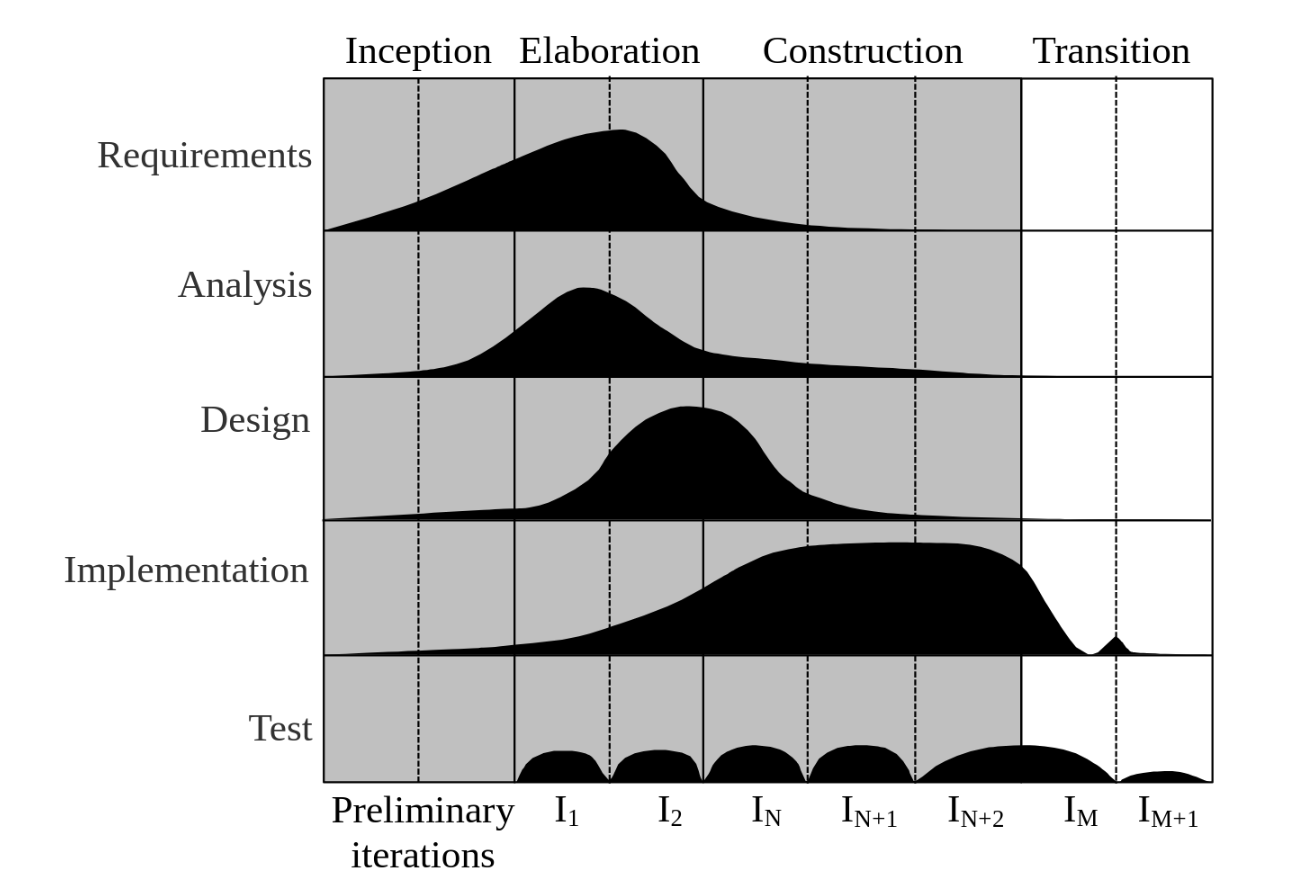
\includegraphics[scale=0.4]{../figures/radit_timeline.png}
\end{center}
dove per ogni fascia associata agli workflow (Requirements, Analysis, ecc...) l'andamento del carico su quel workflow per ogni iterazione ($I_1$, ecc...).

Notiamo come ad esempio la fase di testing diventa parte integrante di ogni iterazione praticamente dalla fase di elaborazione, se non per l'inizio dell'iterazione (dove presumibilmente stiamo progettando/implementando quanto sarà testato).

\subsection{Workflow requisiti}
Il workflow requisiti ha compito di individuare i requisiti del sistema.
Questi sono di due tipi:
\begin{itemize}
	\item \textbf{Funzionali}: legati a \textit{cosa} il sistema deve fare;
	\item \textbf{Non funzionali}: legati a \textit{come} il sistema deve funzionare.
\end{itemize}

Per definire i requisiti in UML possiamo usare un formato molto semplice, del tipo:
\begin{lstlisting}[style=codestyle]	
<id> Il <nome del sistema> deve <funzione da realizzare>
\end{lstlisting}
dove \lstinline|<id>| identifica un requisito.

Quando i requisiti diventano molti, è utile raggrupparli per tipologia. 2 o 3 livelli di profondità della gerarchia sono appropiati finché non si lavora con requisiti particolarmente complessi.

Ogni requisito può essere corredato di uno o più \textit{attributi}, cioè coppie chiave/valore associate al requisito stesso.

\subsubsection{Analisi delle priorità}
L'attributo più comune dei requisiti è la \textbf{priorità}. Questa si definisce secondo l'acronimo \textbf{MoSCoW}, cioè:
\begin{itemize}
	\item \textbf{Must have}: requisiti fondamentali per il sistema;
	\item \textbf{Should have}: requisiti importanti che possono (dopo opportuna discussione) essere omessi;
	\item \textbf{Could have}: requisiti opzionali (da realizzare se possibile, cioè se c'è tmepo);
	\item \textbf{Want to have}: requisiti che non verranno realizzati adesso, ma al massimo in successive release.
\end{itemize}

\subsubsection{Individuazione dei requisiti}
I requisiti sono generati dal contesto di sistema che si vuole modellare, comprensivo di:
\begin{itemize}
	\item Gli utenti del sistema;
	\item Le altre persone coinvolte (installatori, ecc...);
	\item I sistemi con cui il sistema deve interagire; 
	\item I requisiti hardware del sistema e altri vincoli tecnici;
	\item Vincoli legali e regolamenti;
	\item L'obiettivo di business nostro e del cliente.
\end{itemize}

L'individuazione dei requisiti genera solitamente un documento di visione d'insieme, scritto in linguaggio naturale, che delinea i requisiti realizzabili del progetto.

Un processo che possiamo usare è quello di \textit{deduzione} dei requisiti, tecnica dove si cerca di estrarre i requisiti dalle persone coinvolte nel progetto.

Altre metodologie sono le \textit{interviste}, i \textit{questionari} e i \textit{gruppi di lavoro}.

\subsubsection{Modellizzazione casi d'uso}
La \textbf{modellizzazione dei casi d'uso} fa parte dell'ingegnerizzazione dei requisiti, e consiste nell'individuare come gli \textit{attori} (sostanzialmente gli utenti e gli altri elementi coinvolti nell'uso del sistema) interagiscono con questo, all'interno del \textit{soggetto} (il dominio di operazione del sistema). 
\begin{center}
	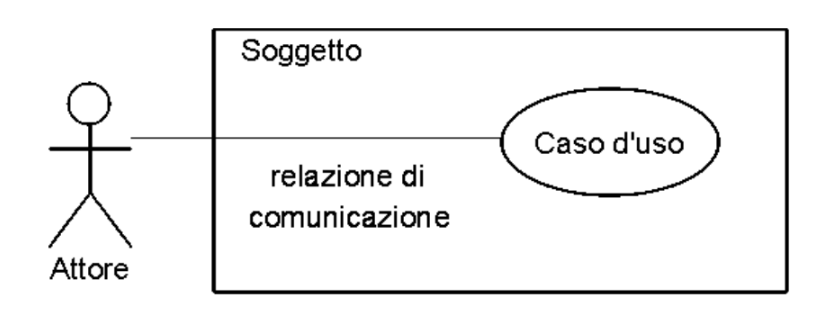
\includegraphics[scale=0.4]{../figures/casi_uso.png}
\end{center}

Questo processo si svolge nel modo seguente:
\begin{itemize}
	\item Identificare un \textit{confine} candidato del sistema, cioè il dominio di operazione del sistema stesso. Identificare il confine del sistema significa capire cosa il sistema è e cosa non è. Questo aiuta nella definizione delle specifiche funzionali.

		In UML i confini del sistema sono chiamati \textbf{soggetto};
	\item Trovare gli \textit{attori} coinvolti nell'uso del sistema, cioè il \textit{ruolo} che le entità esterne assumono quando interagiscono \textit{direttamente} col sistema. 

		Notiamo che nulla vieta che la stessa entità (fisica o astratta) assuma diversi ruoli nell'interazione col sistema. 
		Ad esempio, possiamo pensare a un utente che si comporta sia da utilizzatore che da amministratore di un certo sistema.

		In UML gli \textbf{attori} sono esterni ai \textit{soggetti}. Potrebbe comunque essere che un sistema detiene una rappresentazione interna dell'attore (ad esempio una classe o un record di DB che mantiene i dati dell'utente);
	\item Trovare i \textbf{casi d'uso} del sistema, cioè il tipo di operazioni che il sistema dovrà compiere per conto degli utenti all'interno del suo dominio. A un caso d'uso è associato un \textit{flusso} d'utilizzo del sistema da parte dell'utente. Flussi che divergono dal flusso di default vanno categorizzati e sono detti \textit{flussi alternativi}.
\end{itemize}

\par\smallskip

Vediamo come la modellizzazione dei casi d'uso ci dà una visione d'insieme di come il sistema interagisce, nel suo dominio (\textit{soggetto}) con le parti coinvolte (\textit{attori}):
\begin{center}
	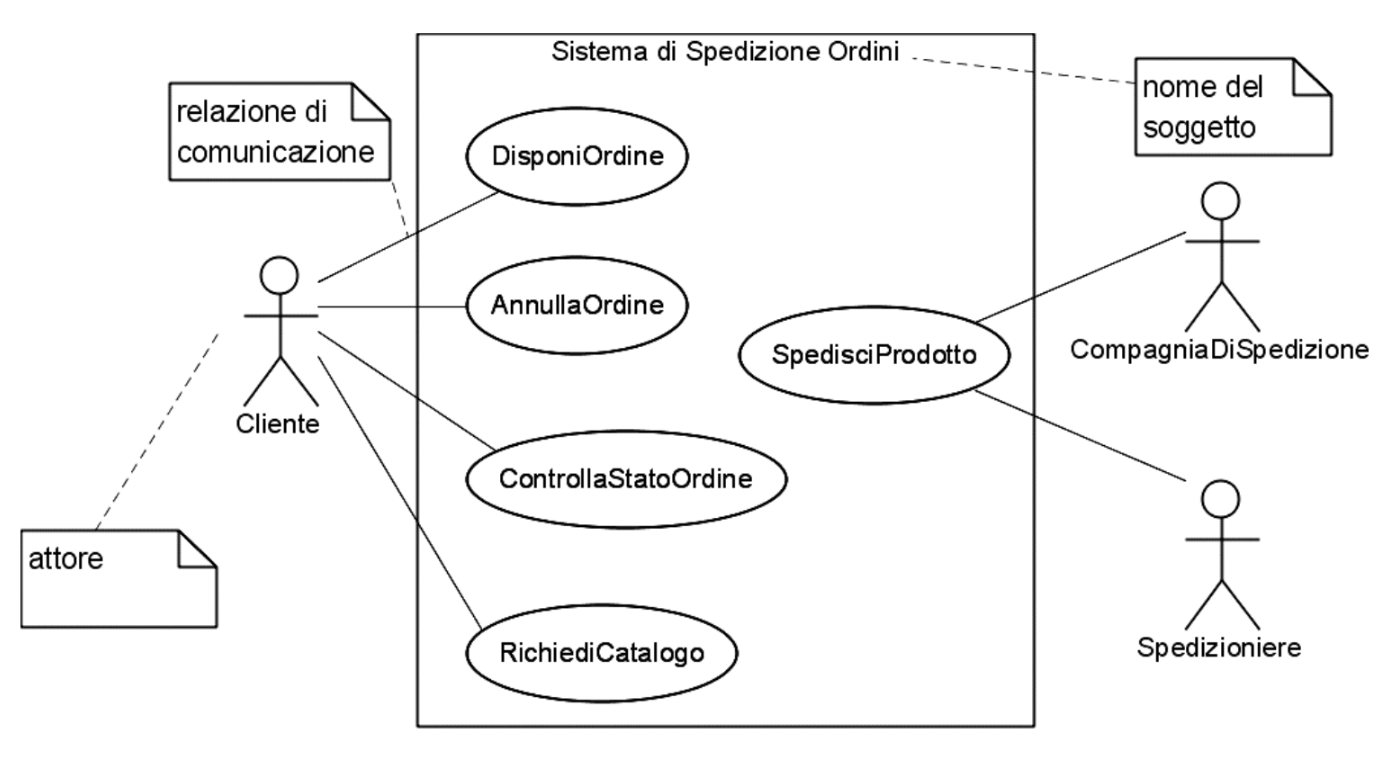
\includegraphics[scale=0.4]{../figures/casi_uso_comp.png}
\end{center}

\subsubsection{Flussi di casi d'uo}
Un caso d'uso è quindi modellizzato attraverso una struttura tabulare che rispecchia la seguente:
\begin{table}[H]
	\center 
	\begin{tabular} { | p{10cm} | }
		\hline
		\bfseries Nome caso d'uso \\ 
		\hline
		Indice \\ 
		\hline
		Descrizione \\ 
		\hline
		Attore primario \\ 
		\hline
		Attori secondari \\ 
		\hline
		Precondizioni \\
		\hline
		\textbf{Flusso principale}:
		\begin{enumerate}
			\item Azione 1;
			\item Azione 2;
			\item ecc...
		\end{enumerate} \\
		\hline
		Postcondizioni \\ 
		\hline
		\textbf{Flussi alternativi}:
		\begin{itemize}
			\item Azione 2 fallita $\rightarrow$ Azione 3;
			\item ecc...
		\end{itemize} \\
		\hline
	\end{tabular}
\end{table}

L'\textbf{indice} è solitamente progressivo (si possono adottare tassonomie, sopratutto nel caso di progetti complessi).

Un caso d'uso è sempre avviato da un singolo attore, l'attore \textbf{primario}. Questo non preclude il fatto che più attori possano avviare lo stesso flusso in momenti diversi. Inoltre, non preclude che altri attori vengano coinvolti: questi saranno gli attori \textbf{secondari}.

Le \textbf{precondizioni} sono le condizioni che devono verificarsi affinché il caso d'uso venga messo in moto, le \textbf{postcondizioni} le condizioni che questo lascerà una volta terminato.

Per definire i casi d'uso in UML usiamo ancora una sintassi molto semplice:
\begin{lstlisting}[style=codestyle]	
Il caso d'uso inizia quando un <attore> <funzione>
\end{lstlisting}

Il flusso di eventi è a questo punto una sequenza (nel caso più semplice):
\begin{lstlisting}[style=codestyle]	
<numero> Il <attore o altro> <azione>
\end{lstlisting}
Vediamo come è possibile prevedere dei \textbf{flussi alternativi} rispetto al \textbf{flusso principale} del caso d'uso. Questo permette una modellazione di comportamenti di errore, eccezioni, o semplici anomalie del flusso principale che si vogliono modellizzare.
Per flussi più complicati ci è concesso usare altri costrutti più tipici della programmazione strutturata, cioè:
\begin{itemize}
	\item Costrutti di ripetizione (\lstinline|for|, \lstinline|while|, ecc...);
	\item Costrutti condizionali (\lstinline|if|, ecc...).
\end{itemize}

I flussi alternativi possono attivarsi in 3 modi differenti:
\begin{itemize}
	\item Per scelta deliberata dell'attore principale;
	\item Attivato dopo un passo del flusso principale, in questo caso si specifica:
\begin{lstlisting}[style=codestyle]	
Il flusso alternativo comincia dopo il passo <numero> del flusso principale
\end{lstlisting}
	\item Attivato ad un passo qualsiasi del flusso principale, in questo caso si specifica:
\begin{lstlisting}[style=codestyle]	
Il flusso alternativo comincia in qualsiasi momento 
\end{lstlisting}
\end{itemize}

Chiaramente, in ogni caso deve esserci una condizione che si verifica perché il flusso alternativo cominci.

\subsubsection{Confronto fra requisiti e casi d'uso}
Una volta terminata l'analisi dei requisiti e dei casi d'uso, si può procedere a stabilire le relazioni che collegano queste 2 categorie (una relazione molti a molti).
Strumento utile in questo caso è la \textbf{matrice di tracciabilità}:

\begin{center}
\raisebox{0pt}{\rotatebox{90}{Requisiti}}
\begin{tabular}[b]{| c | c | c |}
  \multicolumn{3}{c}{Casi d'uso} \\
	\hline
	X & & X \\
	\hline
		& X & \\
		\hline
		& & X \\
	 \hline
\end{tabular}
\end{center}

\subsubsection{Glossario di progetto}
Il \textit{glossario di progetto} è uno dei deliverable principali della fase di ingegnerizzazione dei requisiti.
Questo fornisce un dizionario di termini chiave e definizioni usate nel dominio di applicazione, comprensibili a chiunque sia coinvolto nel progetto.
Di fondamentale importanza è individuare i \textbf{sinonimi}, che potrebbero essere innumerevoli e non apparentemente equivalenti.
Non meno importanti sono gli \textbf{omonimi}, cioè parole uguali usate con significati diversi. 

\par\smallskip

Un esempio di glossario di progetto, riferito ad un sistema per la gestione dei prospetti di laurea, potrebbe essere il seguente:
\begin{center}
	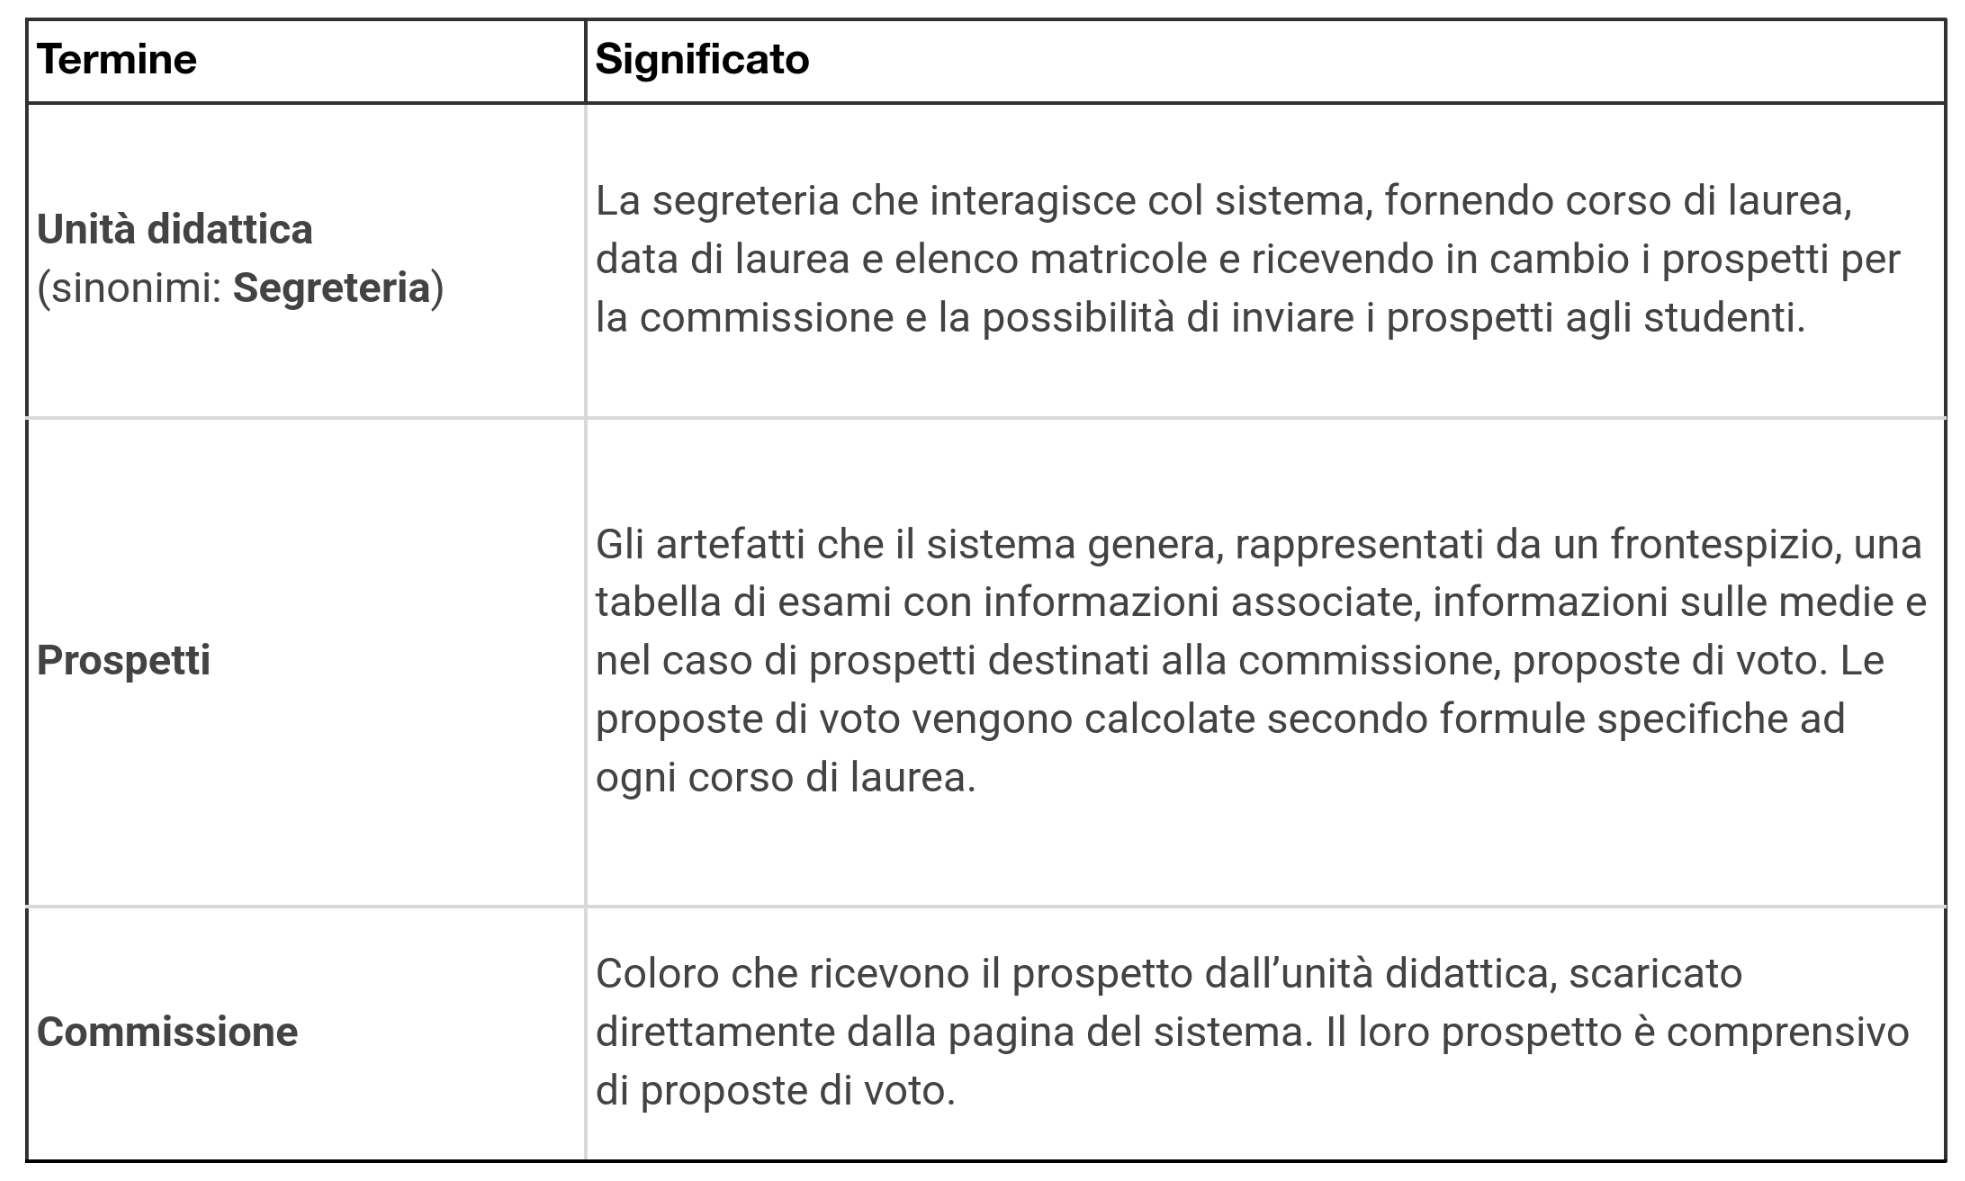
\includegraphics[scale=0.28]{../figures/glossario.png}
\end{center}

\end{document}
